%%%%%%%%%% NJIT 南京工程学院latex模板 2025v1.0.4 %%%%%%%%%%
%v1.0.1---按照最新要求调整了封面格式;优化了目录结构,使其更紧凑;增加学版权授权书,优化结构,方便使用
%v1.0.2---加入字体文件,避免部分编译器不支持模板字体;合并工科/文科模板,便于自由选择封面,因此改为“南京工程学院毕业论文模板”
%v1.0.3---添加研究生模板,优化排版布局,使其更紧凑
%v1.0.4---添加研究生胶皮封面
%%%%%%%%%% Azidiazide azide 3162572053@qq.com %%%%%%%%%%
%%%%%%%%%% 请使用XeLaTeX进行编译 %%%%%%%%%%
\documentclass[a4paper]{njit}
\begin{document}

%%%%%%%%%% 封面,页眉(工科|文科|硕士)选择 %%%%%%%%%%
%封面见njit.cls 147行
%页眉见njit.cls 41行
%注意,硕士学位论文封面位于coverfront.tex,内容可以修改。由于documentclass只能声明一次,因此封面文件需要自行编译为coverfront.pdf
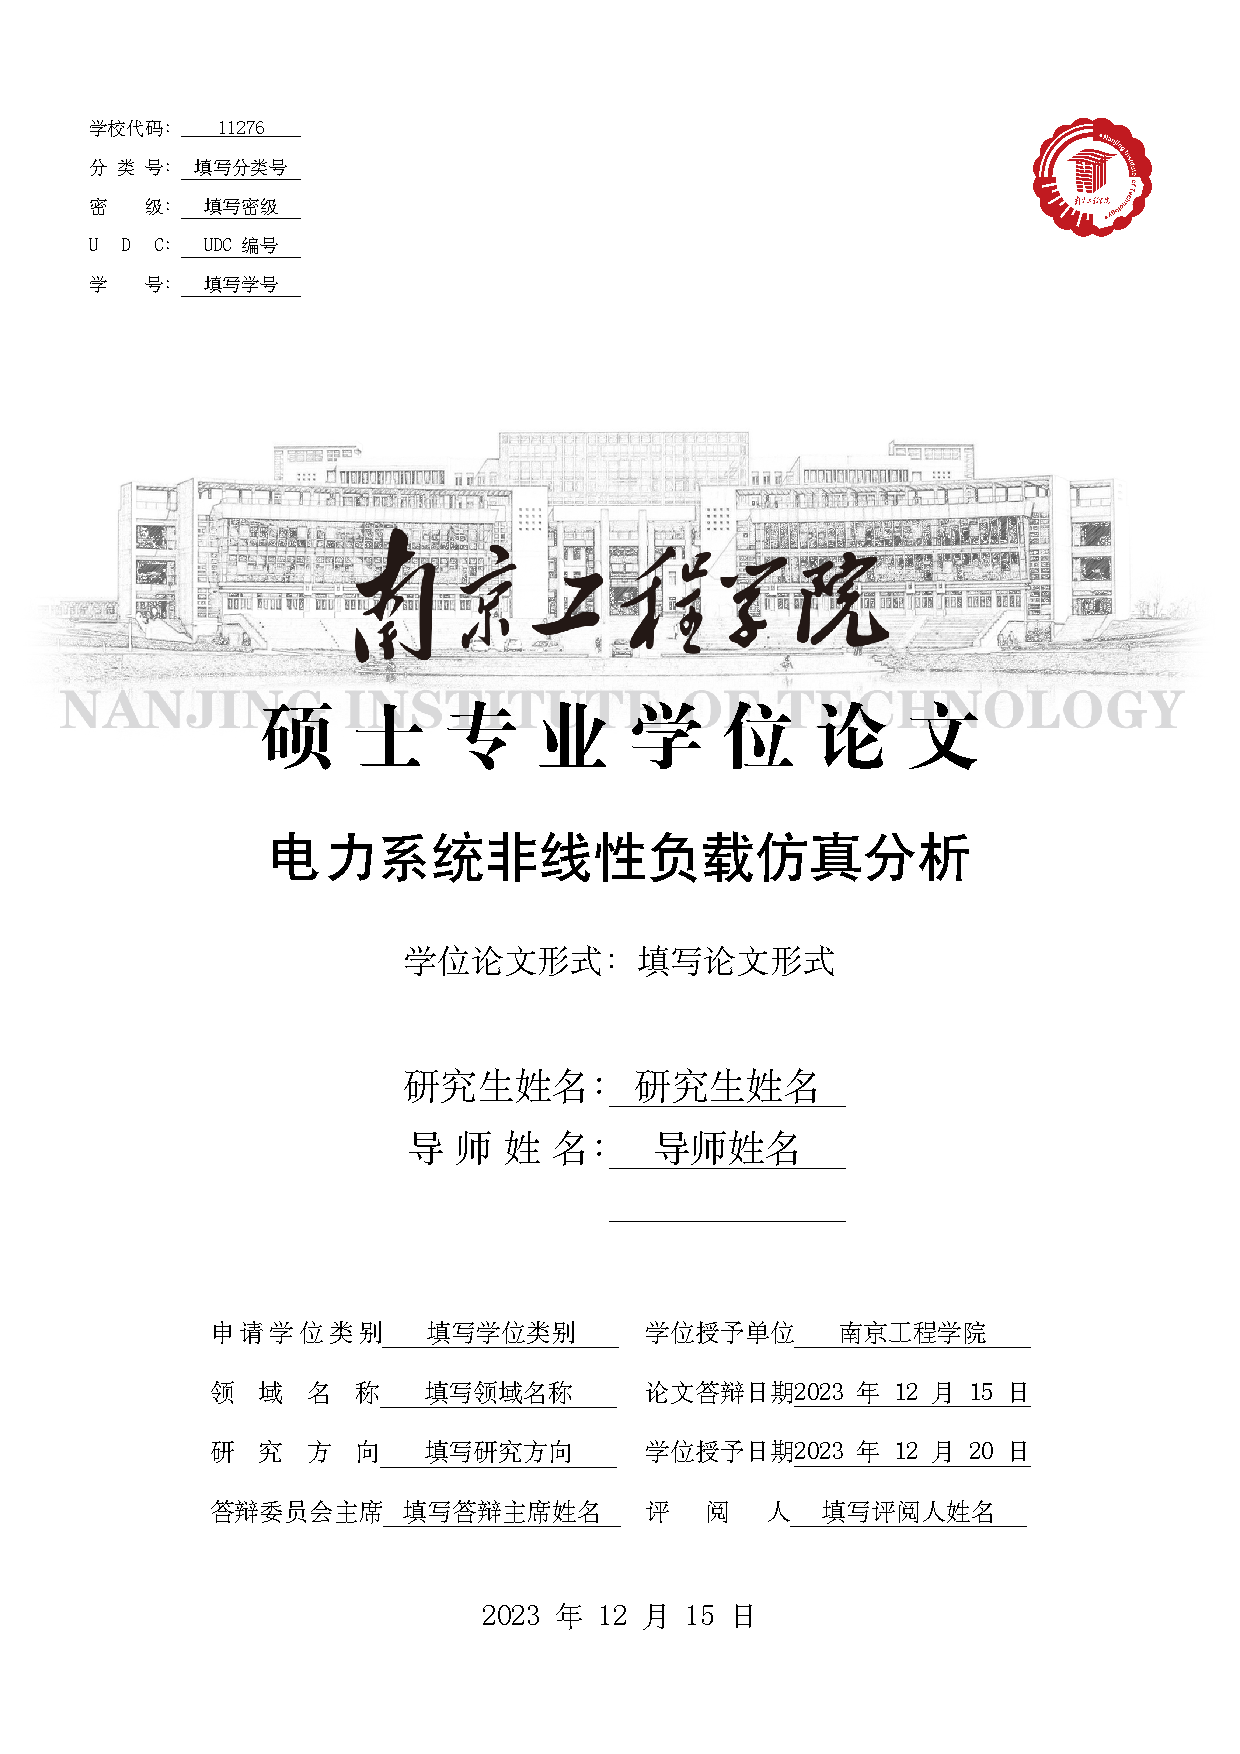
\includepdf{coverfront.pdf} %插入胶皮封面
%%%%%%%%%% 封面,页眉(工科|文科|硕士)选择 %%%%%%%%%%

%%%%%%%%%% 封面 %%%%%%%%%%
\cover
{\LaTeX}                         % 作者
{2025520}                        % 学号
{南京工程学院}                     % 单位
{化学化工学院}                     % 专业
{电力系统非线性负载仿真分析}               % 题目
{及其模拟发生装置研究}                    % 题目
{NJIT \quad \LaTeX 模板}          % 指导者
{}                               % 评阅者
{二〇二五\hspace{0.4em}年\hspace{0.4em}七\hspace{0.4em}月} % 日期

%\newpage
\thispagestyle{empty}

\begin{center}
    \vspace*{1cm}
    
    {\songti \zihao{2} \textbf{Research on Simulation Analysis of Nonlinear Load and Simulation Generating Equipments in Power System}}
    
    \vspace{2cm}
    
    {\zihao{-3} \textbf{A Thesis Submitted to}} \\
    \vspace{0.5cm}
    {\zihao{-3} \textbf{Nanjing Institute of Technology}} \\
    \vspace{0.5cm}
    {\zihao{-3} \textbf{For the professional Degree of Master}}
    
    \vspace{2.5cm}
    
    {\zihao{3} BY XXX} \\
    \vspace{1.5cm}
    {\zihao{3} Supervised by } \\
    \vspace{0.3cm}
     {\zihao{3} Professor XXX} \\
    \vspace{0.3cm}
    {\zihao{3} And}
    
    \vspace{0.3cm} {\zihao{3} Chief Engineer XXX}
    
    \vspace{3cm}
    
    {\zihao{3} School of Electric Power Engineering} \\
    \vspace{0.3cm}
    {\zihao{3} Nanjing Institute of Technology} \\
    \vspace{0.3cm}
    {\zihao{3} January 2025}
    
\end{center}
\newpage

 %英文封面(硕士)
%%%%%%%%%% 封面 %%%%%%%%%%


%%%%%%%%%% 学位论文版权使用授权书 %%%%%%%%%%
\newpage
\thispagestyle{empty}
% 核心命令定义
\newcommand{\thesisdeclaration}[9]{%
\begin{center}
    \zihao{3}\songti \textbf{独创性声明}
\end{center}

\zihao{-4} \songti \textbf{本人}声明所呈交的学位论文是本人在导师指导下进行的研究工作及取得的研究成果,除了文中特别加以标注和致谢之处外,论文中不包含其他人已经发表或撰写过的研究成果,也不包含为获得{\kaishu \zihao{4} \textbf{\underline{\hspace{0.4em}南京工程学院\hspace{0.2em}}}}或其他教育机构的学位或证书而使用过的材料。与我一同工作的同志对本研究所做的任何贡献均已在论文中作了明确的说明并表示了谢意。

\vspace{1.2cm} % 减少垂直间距

\noindent 学位论文作者签名:\underline{\makebox[3cm]{#1}} \hfill 
签字日期:\underline{\makebox[1.2cm]{#2}}年\underline{\makebox[0.8cm]{#3}}月\underline{\makebox[0.8cm]{#4}}日

\vspace{1.5cm} % 减少间距

\begin{center}
    \zihao{3} \songti \textbf{学位论文版权使用授权书}
\end{center}

\zihao{-4} \songti 本学位论文作者完全了解{\kaishu \zihao{4} \textbf{\underline{\hspace{0.4em}南京工程学院\hspace{0.2em}}}}有关保留、使用学位论文的规定。特授权{\kaishu \zihao{4} \textbf{\underline{\hspace{0.4em}南京工程学院\hspace{0.2em}}}}可以将学位论文的全部或部分内容编入有关数据库进行检索,并采用影印、缩印或扫描等复制手段保存、汇编以供查阅和借阅。同意学校向国家有关部门或机构送交论文的复印件和磁盘。\\

{\centering \songti \textbf{(保留的学位论文在解密后适用本授权说明)} \\}



\vspace{1.2cm}

\noindent 学位论文作者签名:\underline{\makebox[3cm]{#1}}  \hspace{2cm} 
导师签名:\underline{\makebox[3.5cm]{#5}}

\vspace{0.6cm}

\noindent 签字日期:\underline{\makebox[1.2cm]{#2}}年\underline{\makebox[0.8cm]{#3}}月\underline{\makebox[0.8cm]{#4}}日 \hspace{2.5cm}
签字日期:\underline{\makebox[1.2cm]{#6}}年\underline{\makebox[0.8cm]{#7}}月\underline{\makebox[0.8cm]{#8}}日

\vspace{4cm}
\begin{center}
论文提交日期:\underline{\makebox[6cm]{#9}}
\end{center}
}


 %本科(二选一注释即可)
%\newpage
\thispagestyle{empty}
% 核心命令定义
\newcommand{\thesisdeclaration}[9]{%
\begin{center}
    \zihao{3}\songti \textbf{南京工程学院学位论文独创性声明}
\end{center}

\zihao{-4} \songti \textbf{本人}声明所呈交的学位论文是本人在导师指导下进行的研究工作及取得的研究成果,除了文中特别加以标注和致谢之处外,论文中不包含其他人已经发表或撰写过的研究成果,也不包含为获得{\kaishu \zihao{4} \textbf{\underline{\hspace{0.4em}南京工程学院\hspace{0.2em}}}}或其他教育机构的学位或证书而使用过的材料。与我一同工作的同志对本研究所做的任何贡献均已在论文中作了明确的说明并表示了谢意。

\vspace{1.2cm} % 减少垂直间距

\noindent 研究生签名:\underline{\makebox[2cm]{#1}} \hfill 
签字日期:\underline{\makebox[1.2cm]{#2}}年\underline{\makebox[0.8cm]{#3}}月\underline{\makebox[0.8cm]{#4}}日

\vspace{1.5cm} % 减少间距

\begin{center}
    \zihao{3} \songti \textbf{南京工程学院学位论文使用授权声明}
\end{center}

\zihao{-4} \songti 南京工程学院、中国科学技术信息研究所、国家图书馆有权保留本人所送交学位论文的复印件和电子文档,可以采用影印、缩印或其他复制手段保存论文。本人电子文档的内容和纸质论文的内容相一致。除在保密期内的保密论文外,允许论文被查阅和借阅,可以公布(包括刊登)论文的全部或部分内容。论文的公布(包括刊登)授权南京工程学院研究生院办理。\\

{\centering \songti \textbf{(保留的学位论文在解密后适用本授权说明)} \\}



\vspace{1.2cm}

\noindent 研究生签名:\underline{\makebox[2cm]{#1}}  \hspace{0cm} 
导师签名:\underline{\makebox[2cm]{#5}}\hspace{0cm} 签字日期:\underline{\makebox[1.2cm]{#2}}年\underline{\makebox[0.8cm]{#3}}月\underline{\makebox[0.8cm]{#4}}日



\vspace{4cm}
\begin{center}
论文提交日期:\underline{\makebox[6cm]{#9}}
\end{center}
}


 %硕士
\thesisdeclaration
{张三}        % #1 作者
{2025}        % #2 作者年
{07}          % #3 作者月
{15}          % #4 作者日
{李四}        % #5 导师
{2025}        % #6 导师年
{07}          % #7 导师月
{20}          % #8 导师日
{二〇二五年七月二十五日} % #9 提交日期
\newpage
%%%%%%%%%% 学位论文版权使用授权书 %%%%%%%%%%


%%%%%%%%%% 封面目录摘要 %%%%%%%%%%
\pagestyle{plain}
\pagenumbering{Roman} 
%%%%%%%%%% 中文摘要部分 %%%%%%%%%%
\thispagestyle{empty} % 当前页不显示页眉页脚
\begin{center}
    \vspace*{-1.4cm} % 调整垂直位置
    {\zihao{-2}\songti \textbf{毕\hspace{0.3em}业\hspace{0.3em}设\hspace{0.3em}计\hspace{0.3em}说\hspace{0.3em}明\hspace{0.3em}书\hspace{0.3em}(论文)\hspace{0.3em}中\hspace{0.3em}文\hspace{0.3em}摘\hspace{0.3em}要}}\\
\end{center}

\begin{tikzpicture}[remember picture, overlay]
    \draw[line width=1pt] 
        (current page.north west) ++(2.8cm,-3.5cm) rectangle 
        ++(\dimexpr\paperwidth-2.8cm-2.4cm, -\dimexpr\paperheight-3.5cm-2.6cm);
\end{tikzpicture}

\setlength{\parindent}{2em}   % 段首空两格
\setlength{\parskip}{0pt plus 1.0pt}    % 段间距
\zihao{-4}\songti             % 统一设置为小四宋体


% --- 摘要部分 ---
\vspace*{-30pt}
\begin{center}
    \zihao{3}\heiti \textbf{摘\quad 要}
\end{center}
\vspace*{-10pt}


 岩沙海葵毒素的首次全合成由哈佛大学岸义人团队历经近二十年最终完成。面对这一结构异常庞大且复杂的天然产物,核心策略是将其逆向分解为八个相对易于合成的关键片段,分别标记为片段A至片段H。这些片段的划分依据了分子内天然存在的重复结构单元,例如连续的1,3-二醇片段以及特定的烯烃链段,旨在简化合成路径并有效控制立体化学。

 每个关键片段的合成本身就是一个复杂的工程,需要精心设计与执行。片段A涵盖了分子的C1至C15部分,片段B对应C16至C26,片段C对应C27至C38。片段D则更为复杂,包含了C39至C51以及C68至C70区域,其核心结构是一个内半缩醛。片段E和F分别负责构建C52至C67和C71至C78的链段。片段G连接了C79至C98部分,而最大且最富挑战性的片段H则构建了分子的末端,包括C99至C129,这一片段包含了关键的酰胺结构。

 成功合成这些片段后,接下来的核心挑战在于如何高立体选择性地将这些“积木”精确无误地连接起来。团队发展并应用了一系列精密的片段偶联反应来实现这一目标。例如,通过Wittig烯化反应连接片段C和D,构建了C38-C39键。片段D和E则是通过醛醇缩合反应在C51-C52位置实现连接。片段F和G的连接采用了Sharpless不对称环氧化和随后的环氧开环策略在C78-C79处进行偶联。而构建C98-C99键的关键步骤则是通过片段G和H的醛醇缩合反应完成的。片段B和C的连接以及A和B的连接也分别运用了醛醇缩合和Wittig烯化反应。

在整个组装过程中,如何精确控制每一步新生成的手性中心的立体化学是贯穿始终的难题。团队巧妙地利用了多种策略,包括Evans手性辅基诱导的不对称合成、高选择性的Sharpless不对称环氧化反应、底物自身的手性诱导效应以及经过严格优化的反应条件,最终成功地在超过六十四个手性中心上实现了所需的绝对和相对立体构型。整个合成路线共经历了一百二十余步反应,最终以毫克级的规模成功获得了目标产物,充分展现了合成设计的前瞻性、立体控制技术的精湛以及复杂多步操作的无缝衔接,成为有机合成史上的一个巅峰成就。

% 关键词部分
\vspace{0.5cm}
\noindent
\zihao{-4}\heiti 关键词:\zihao{-4}\songti 不对称合成;环氧化反应;片段偶联;Wittig烯化


\newpage % 分页
%%%%%%%%%% 英文摘要部分 %%%%%%%%%%
\thispagestyle{empty} % 当前页不显示页眉页脚
\begin{center}
    \vspace*{-1.6cm} % 调整垂直位置
    {\zihao{-2}\songti \textbf{毕\hspace{0.3em}业\hspace{0.3em}设\hspace{0.3em}计\hspace{0.3em}说\hspace{0.3em}明\hspace{0.3em}书\hspace{0.3em}(论文)\hspace{0.3em}外\hspace{0.3em}文\hspace{0.3em}摘\hspace{0.3em}要}}\\
\end{center}
\begin{tikzpicture}[remember picture, overlay]
    \draw[line width=1pt] 
        (current page.north west) ++(2.8cm,-3.5cm) rectangle 
        ++(\dimexpr\paperwidth-2.8cm-2.4cm, -\dimexpr\paperheight-3.5cm-2.6cm);
\end{tikzpicture}

\setlength{\parindent}{2em}   % 段首空两格
\setlength{\parskip}{0pt plus 1.0pt}   % 段间距
\zihao{-4}\songti             % 统一设置为小四宋体


% --- 摘要部分 ---
\vspace*{-30pt}
\begin{center}
    \zihao{3}\heiti \textbf{Abstract}
\end{center}
\vspace*{-10pt}


 The first total synthesis of anemone toxin in rock sand was finalized by the team of Yoshito Kishi at Harvard University over a period of nearly two decades. Faced with this unusually large and complex natural product, the core strategy is to reverse decompose it into eight critical fragments that are relatively easy to synthesize, labeled as fragments A to H. The division of these fragments is based on the naturally occurring repeating structural units within the molecule, such as successive 1,3-diol fragments, as well as specific olefin segments, with the aim of simplifying the synthetic pathway and effectively controlling stereochemistry.

 The synthesis of each critical segment is a complex project in itself, requiring careful design and execution. Fragment A covers the C1 to C15 portion of the molecule, with fragment B corresponding to C16 to C26 and fragment C corresponding to C27 to C38. Fragment D is more complex, containing regions C39 to C51 and C68 to C70, with an inner hemiacetal at its core. Fragments E and F are responsible for the construction of segments C52 to C67 and C71 to C78, respectively. Fragment G connects the C79 to C98 moieties, while the largest and most challenging fragment H constructs the ends of the molecule, including C99 to C129, which contains the key amide structure.




% 关键词部分
\vspace{0.5cm}
\noindent
\zihao{-4}\heiti \textbf{Keywords}:\zihao{-4}\songti asymmetric synthesis; epoxidation reaction; fragment conjugation; Wittig enylation



%\clearpage 
%\mytableofcontents %目录部分
%\clearpage  

\clearpage
\thispagestyle{fancy} % 强制当前页显示页眉
\begin{spacing}{1}
    \tableofcontents
\end{spacing}
\thispagestyle{fancy} % 确保下一页页眉正常
\newpage %本科
%\newgeometry{left=2cm, right=2cm, top=2.5cm, bottom=2.5cm}

\newcommand{\fakeheader}[1]{%
    \vspace*{-2cm}
    \begin{center}
        \zihao{-5}\songti #1\\[-10pt] 
        \rule{\textwidth}{0.4pt} 
    \end{center}
    \vspace{-0.5cm} 
}

\renewcommand{\abstractname}{\songti \zihao{3}\heiti 摘\quad 要}
\renewcommand{\absnamepos}{center}


\newcommand{\enabstractname}{\songti \zihao{3}\textbf{ABSTRACT}}
\newenvironment{englishabstract}{%
    \renewcommand{\abstractname}{\enabstractname}
    \begin{abstract}
}{%
    \end{abstract}
}

\date{}
\pagenumbering{Roman} 


% ========== 中文摘要 ==========
\fakeheader{摘要} 
\begin{abstract}
    \thispagestyle{plain}
    
    \setlength{\parindent}{2em}
    \setlength{\baselineskip}{20pt}

   \songti \zihao{-4}本文研究了电力系统中非线性负载及仿真发电设备的建模与仿真分析方法。首先,基于\ldots(此处填写摘要内容,300字左右)。针对\ldots 问题,提出了\ldots 方法。实验结果表明,所提方法能有效\ldots(结论)。本研究对\ldots 具有重要意义。
    
    \vspace{1em}
    {\noindent\heiti 关键词:} 电力系统;非线性负载;仿真建模;谐波分析
\end{abstract}

\newpage
\newcommand{\header}[1]{%
    \vspace*{-2cm} 
    \begin{center}
        \zihao{-5}\songti #1\\[-10pt] 
        \rule{\textwidth}{0.4pt}
    \end{center}
    \vspace{-0.5cm} 
}

% ========== 英文摘要 ==========
\header{南京工程学院硕士专业学位论文}
\begin{englishabstract} % 使用自定义的英文摘要环境
    \thispagestyle{plain}
    
    \setlength{\parindent}{0em}
    \setlength{\baselineskip}{20pt}
    
    \songti \zihao{-4} This paper investigates the modeling and simulation analysis methods for nonlinear loads and simulation generating equipment in power systems. Firstly, \ldots (英文摘要内容,与中文对应). To address \ldots, a \ldots method is proposed. Experimental results show that \ldots (结论). This study is significant for \ldots.
    
    \vspace{1em}
    {\noindent \textbf{Keywords:}} power system; nonlinear load; simulation modeling; harmonic analysis
\end{englishabstract}
\restoregeometry




\clearpage
\thispagestyle{fancy} % 强制当前页显示页眉
\begin{spacing}{1}
    \tableofcontents
\end{spacing}
\thispagestyle{fancy} % 确保下一页页眉正常
\newpage


 %研究生
\pagestyle{fancy}
%%%%%%%%%% 封面目录摘要 %%%%%%%%%%

%%%%%%%%%% 正文 %%%%%%%%%%
\pagenumbering{arabic}

\section{绪言}

\subsection{\LaTeX 介绍}

要使用 \LaTeX{} 来完成建模论文,首先要确保正确安装一个 \LaTeX{} 的发行版本。

\begin{itemize}
    \item Mac 下可以使用 Mac\TeX{}
    \item Linux 下可以使用 \TeX{}Live ;
    \item windows 下可以使用 \TeX{}Live 或者 Mik\TeX{} ;
\end{itemize}

具体安装可以参考 \href{https://github.com/OsbertWang/install-latex-guide-zh-cn/releases/}{Install-LaTeX-Guide-zh-cn} 或者其它靠谱的文章。另外可以安装一个易用的编辑器,例如 \href{https://mirrors.tuna.tsinghua.edu.cn/github-release/texstudio-org/texstudio/LatestRelease/}{\TeX{}studio} 。


\subsection{本模板介绍}

为简化南京工程学院本科生毕业论文排版流程,开发了符合校标的LaTeX模板。该模板内置最新格式规范,可自动处理页眉页脚、标题样式、参考文献等排版要素,使用者仅需编写内容即可生成标准化文档,有效提升写作效率并确保格式统一性。

使用该模板前,请阅读模板的使用说明文档。下面给出模板使用的大概样式。

\subsubsection{文档类的选取}

模版的文档类是基于\CTeX{} 宏集中自带的ctexart文档类来实现的\cite{x5},还用到了一些常用的宏包,编译时要保证自己的系统中已经安装好了这些宏包,如果用户使用的是全量安装的 TeX Live就没有问题。

\subsubsection{参考文献编译方式}

模板推荐使用\verb|\bibliography{}|命令处理参考文献,借助“GB/T 7714—2015 BibTeX Style”\cite{x6},模板使用者可以放心大胆地将参考文献的排版工作交给\LaTeX ,而无需手动调整每条参考文献的格式。

编译记得使用 \verb|xelatex|,而不是用 \verb|pdflatex|。在命令行编译的可以按如下方式编译:
\begin{tcode}
	xelatex example
\end{tcode}
或者使用 \verb|latexmk| 来编译,更推荐这种方式。
\begin{tcode}
	latexmk -xelatex example
\end{tcode}

下面给出写作与排版上的一些建议\footnote{部分内容摘自《全国大学生数学建模\LaTeX》}。
\section{图片}


论文中不可避免要插入图片。图片可以分为矢量图与位图。位图推荐使用 \verb|jpg,png| 这两种格式,避免使用 \verb|bmp| 这类图片,容易出现图片插入失败这样情况的发生。矢量图一般有 \verb|pdf,eps| ,推荐使用 \verb|pdf|  格式的图片,尽量不要使用 \verb|eps| 图片,理由相同。

注意图片的命名,避免使用中文来命名图片,可以用英文与数字的组合来命名图片。避免使用\verb|1,2,3| 这样顺序的图片命名方式。图片多了,自己都不清楚那张图是什么了,命名尽量让它有意义。下面是一个插图的示例代码。
\begin{figure}[!h]
    \centering
    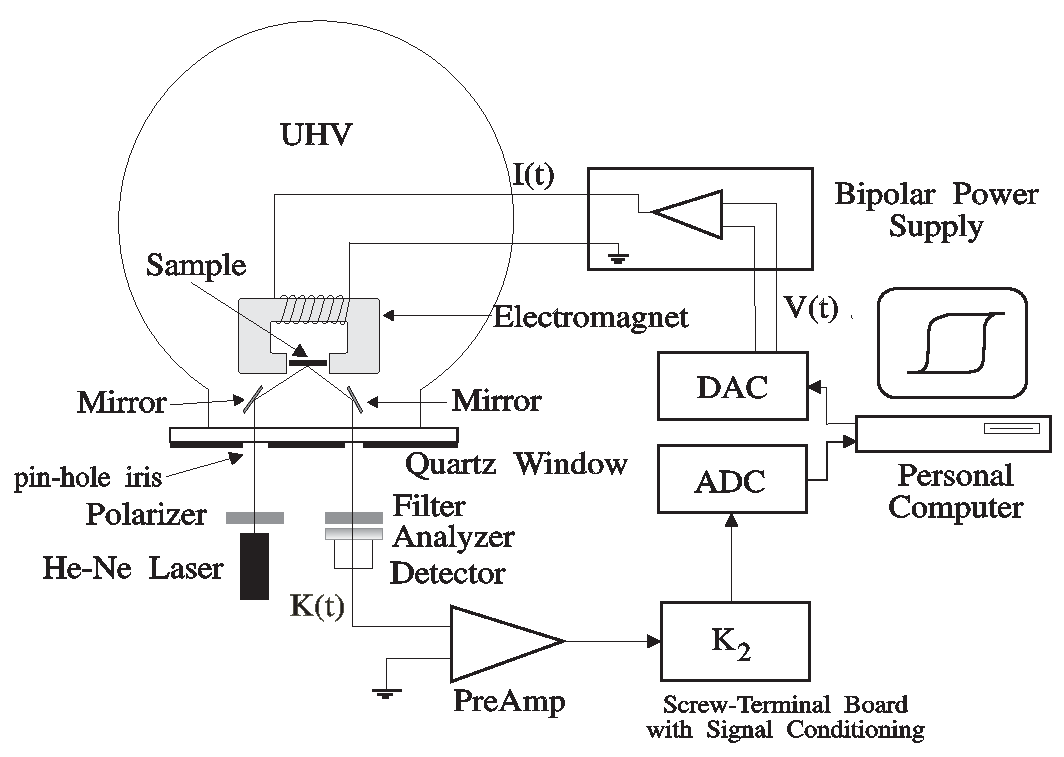
\includegraphics[width=.6\textwidth]{figures/smokeblk.pdf}
    \caption{电路图}
    \label{figures:smokeblk.pdf}
\end{figure}

注意 \verb|figure| 环境是一个浮动体环境,图片的最终位置可能会跑动。\verb|[!h]| 中的 \verb|h| 是 here 的意思, \verb|!| 表示忽略一些浮动体的严格规则。另外里面还可以加上 \verb|btp| 选项,它们分别是 bottom, top, page 的意思。只要这几个参数在花括号里面,作用是不分先后顺序的。page 在这里表示浮动页。

\verb|\label{fig:circuit-diagram}| 是一个标签,供交叉引用使用的。图片是自动编号的,比起手动编号,它更加高效。\verb|\cref{label}| 由 \verb|cleveref| 宏包提供,比普通的 \verb|\ref{label}| 更加自动化。 \verb|label| 要确保唯一,命名方式推荐用图片的命名方式。

图片并排的需求解决方式多种多样,下面用 \verb|minipage| 环境来展示一个简单的例子。注意,以下例子用到了 \verb|subcaption| 命令,需要加载 subcaption 宏包。

\begin{figure}
    \centering
    \begin{minipage}[c]{0.3\textwidth}
        \centering
        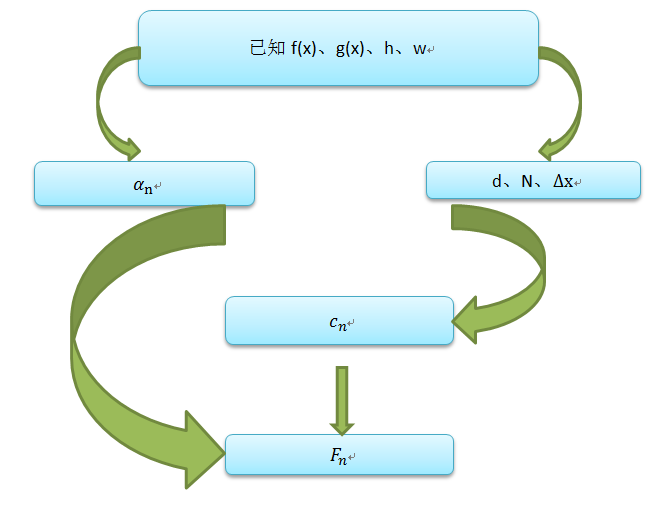
\includegraphics[width=0.95\textwidth]{figures/f1.png}
        \subcaption{流程图}
        \label{fig:sample-figure-a}
    \end{minipage}
    \begin{minipage}[c]{0.3\textwidth}
        \centering
        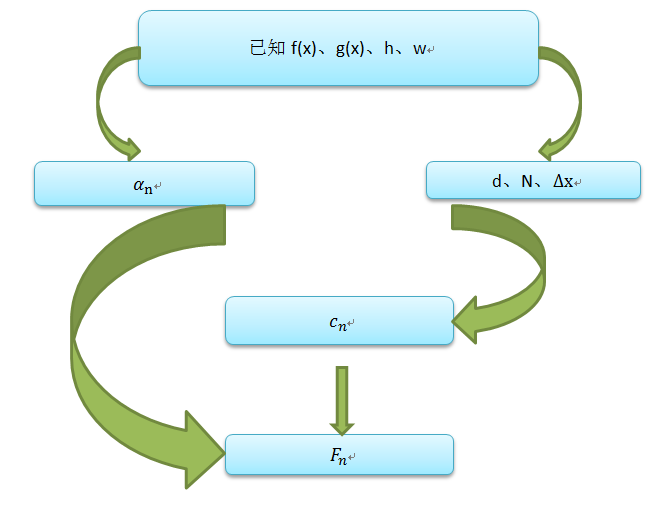
\includegraphics[width=0.95\textwidth]{figures/f1.png}
        \subcaption{流程图}
        \label{fig:sample-figure-b}
    \end{minipage}
    \begin{minipage}[c]{0.3\textwidth}
        \centering
        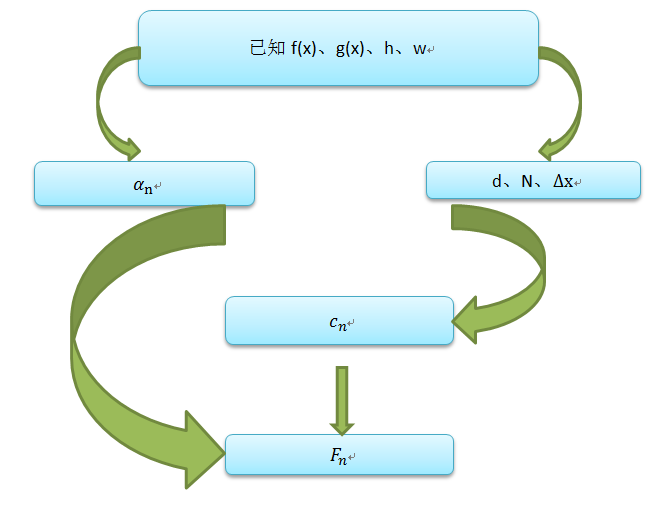
\includegraphics[width=0.95\textwidth]{figures/f1.png}
        \subcaption{流程图}
        \label{fig:sample-figure-c}
    \end{minipage}
    \caption{多图并排示例}
    \label{fig:sample-figure}
\end{figure}

这相当于整体是一张大图片,大图片引用是\cref{fig:sample-figure},子图引用别分是\cref{fig:sample-figure-a}、\cref{fig:sample-figure-b}、\cref{fig:sample-figure-c}。

如果原本两张图片的高度不同,但是希望它们缩放后等高的排在同一行,参考这个例子:
\begin{figure}[H]
    \centering
    \begin{minipage}[c]{0.4\textwidth}
        \centering
        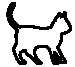
\includegraphics[height=0.2\textheight]{figures/cat.pdf}
        \subcaption{一只猫}
    \end{minipage}
    \begin{minipage}[c]{0.4\textwidth}
        \centering
        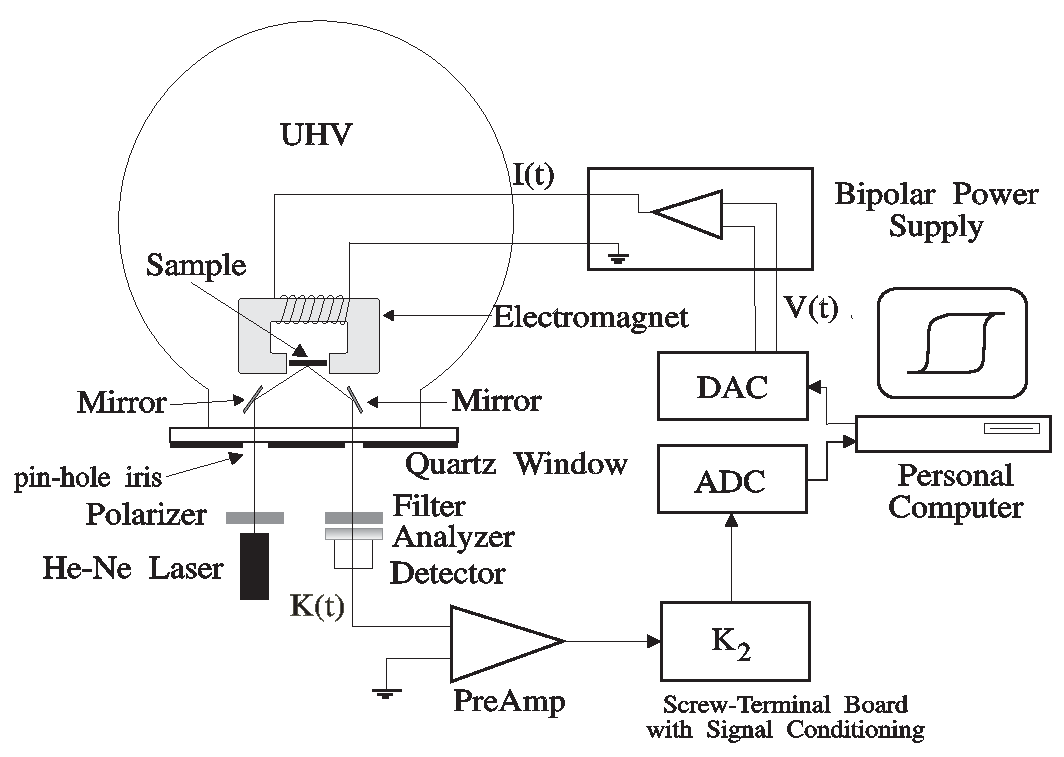
\includegraphics[height=0.2\textheight]{figures/smokeblk.pdf}
        \subcaption{电路图}
    \end{minipage}
    \caption{多图并排示例}
\end{figure}

\section{绘制普通三线表格}

表格应具有三线表格式,因此常用 booktabs宏包,其标准格式如\cref{tab:001}~所示。

\begin{table}[H]
    \caption{标准三线表格}\label{tab:001} \centering
    \vspace{-6pt}
    \begin{tabular}{ccccc}
        \toprule[1.5pt]
        $D$(in) & $P_u$(lbs) & $u_u$(in) & $\beta$ & $G_f$(psi.in)\\
        \midrule[1pt]
        5 & 269.8 & 0.000674 & 1.79 & 0.04089\\
        10 & 421.0 & 0.001035 & 3.59 & 0.04089\\
        20 & 640.2 & 0.001565 & 7.18 & 0.04089\\
        \bottomrule[1.5pt]
    \end{tabular}
\end{table}

其绘制表格的代码及其说明如下。
\begin{tcode}
    \begin{table}[!htbp]
        \caption[标签名]{中文标题}
        \begin{tabular}{cc...c}
            \toprule[1.5pt]
            表头第1个格   & 表头第2个格   & ... & 表头第n个格  \\
            \midrule[1pt]
            表中数据(1,1) & 表中数据(1,2) & ... & 表中数据(1,n)\\
            表中数据(2,1) & 表中数据(2,2) & ... & 表中数据(2,n)\\
            ...................................................\\
            表中数据(m,1) & 表中数据(m,2) & ... & 表中数据(m,n)\\
            \bottomrule[1.5pt]
        \end{tabular}
    \end{table}
\end{tcode}

\bigskip

table环境是一个将表格嵌入文本的浮动环境。tabular环境的必选参数由每列对应一个格式字符所组成:c表示居中,l表示左对齐,r表示右对齐,其总个数应与表的列数相同。此外,\verb|@{文本}|可以出现在任意两个上述的列格式之间,其中的文本将被插入每一行的同一位置。表格的各行以\verb|\\|分隔,同一行的各列则以\&分隔。 \verb|\toprule| 、\verb|\midrule| 和 \verb|\bottomrule| 三个命令是由booktabs宏包提供的,其中 \verb|\toprule| 和 \verb|\bottomrule| 分别用来绘制表格的第一条(表格最顶部)和第三条(表格最底部)水平线, \verb|\midrule| 用来绘制第二条(表头之下)水平线,且第一条和第三条水平线的线宽为 1.5pt ,第二条水平线的线宽为 1pt 。引用方法与图片的相同。

这里笔者给出常见用法,以供参考。

\begin{table}[H]
    \caption{符号说明}
    \vspace{-6pt}
    \centering
    \begin{tabularx}{0.9\textwidth}{c| >{\raggedright\arraybackslash}X}
        \toprule[1.5pt]
        \textbf{符号} & \textbf{内容说明} \\
        \midrule[1pt]
      
        $\epsilon_\mathrm{tol}$ & 算法误差容限 \\
        $\mathbf{a}_\odot^\mathrm{tidal}$ & 太阳引潮力项,按二阶梯度展开计算 \\
        $E$ & 偏近点角,通过牛顿迭代法求解开普勒方程 \\
        $\mathbf{\hat{P}},\mathbf{\hat{Q}}$ & 轨道面正交基向量,由$(\Omega,\omega,i)$计算 \\
        $\mathbf{k}_1,\mathbf{k}_2,...\mathbf{k}_{13}$ & 算法中间系数,对应13次函数估值 \\
        $B_{\mathrm{eff}}$ & 有效摄动阶数 \\
        \bottomrule[1.5pt]
    \end{tabularx}
\end{table}


\begin{table}[H]
\centering
\caption{2028 Olympic Medal Predictions (Top 14 Countries by Total Score)}
\vspace{-6pt} 
\label{tab:top14_medals}
\begin{tabular}{l|ccc|c} % 修正:5列(1左对齐 + 4居中对齐)
\toprule
\textbf{Country} & \textbf{Gold} & \textbf{Silver} & \textbf{Bronze} & \textbf{Total Score} \\
\midrule
United States         & 40.0 (38.0--46.3) & 40.4 (38.4--44.0) & 33.9 (32.2--42.0) & 112.0  \\
China                 & 36.7 (34.9--40.0) & 27.0 (25.6--30.4) & 24.0 (22.8--31.5) & 90.8    \\
Great Britain         & 17.1 (16.2--30.7) & 22.8 (21.7--28.5) & 26.6 (25.3--30.5) & 67.3     \\
Russia                & 14.3 (13.6--23.6) & 18.1 (17.2--20.9) & 20.9 (19.9--20.1) & 55.7    \\
France                & 12.1 (11.5--25.3) & 13.3 (12.6--26.0) & 21.2 (20.1--22.0) & 47.0    \\
Australia             & 12.1 (11.5--22.6) & 14.4 (13.7--19.4) & 16.2 (15.4--16.5) & 46.7    \\
Japan                 & 13.1 (12.4--20.5) & 14.9 (14.2--19.0) & 15.3 (14.5--17.0) & 45.0     \\
Italy                 & 12.1 (11.5--16.4) & 13.0 (12.3--13.6) & 17.4 (16.5--20.8) & 40.2     \\
Germany               & 12.1 (11.5--19.8) & 12.8 (12.2--18.7) & 13.4 (12.7--16.4) & 33.2     \\
Netherlands           & 7.1 (6.7--15.0)   & 8.0 (7.6--11.4)   & 12.8 (12.2--16.3) & 30.8     \\
South Korea           & 7.7 (7.3--13.0)   & 7.9 (7.5--9.5)    & 9.8 (9.3--10.9)   & 29.0    \\
New Zealand           & 4.5 (4.3--10.0)   & 5.9 (5.6--9.7)    & 5.8 (5.5--10.3)   & 20.1     \\
Brazil                & 4.8 (4.6--11.1)   & 6.1 (5.8--9.1)    & 7.4 (7.0--11.3)   & 20.0     \\
Canada                & 5.4 (5.1--10.2)   & 5.6 (5.3--7.3)    & 8.2 (7.8--11.0)   & 19.2    \\
\bottomrule
\end{tabular}
\smallskip
\vspace{2pt}
\footnotesize \textit{Note: Values are formatted as "median (confidence interval)". Countries are ranked by total score median.}
\end{table}


\begin{algorithm}[H]
\caption{预测误差与观测时间算法}
\label{alg:propagation}
\begin{algorithmic}[1]
\Require 
\Statex 初始轨道参数 $\mathbf{X}_0 \in \mathbb{R}^6$ (含误差协方差$\mathbf{P}_0$)
\Statex 摄动力模型 $\mathcal{M}$ (含J2至J6项、日月摄动、太阳光压等)
\Ensure
\Statex 位置误差统计量 $\mu_{\epsilon},\sigma_{\epsilon} \in \mathbb{R}^3$

\Procedure{误差传播分析}{$\mathbf{X}_0, \mathbf{P}_0, T_{max}$}
\State \textbf{步骤1:建立参考轨道}
\State 生成精密星历轨迹:
\quad $\mathbf{X}_{ref}(t) \gets \text{SPICE\_ephem}(t), t\in[0,T_{max}]$
\State 构造变分方程:
\quad $\frac{d}{dt}\Phi(t,0) = \mathbf{A}(t)\Phi(t,0)$

\State \textbf{步骤2:参数扰动采样}
\State 分解协方差矩阵:$\mathbf{P}_0 = \mathbf{L}\mathbf{L}^\top$ 
\For{$k=1$ \textbf{to} $N_{MC}$}
    \State 生成随机扰动:$\delta\mathbf{X}_k \gets \mathbf{L}\mathbf{z}_k,\ \mathbf{z}_k \sim \mathcal{N}(0,1)$
    \State 样本轨道参数:$\mathbf{X}_k^{(0)} \gets \mathbf{X}_0 + \delta\mathbf{X}_k$
\EndFor

\State \textbf{步骤3:轨道传播计算}
\For{$k=1$ \textbf{to} $N_{MC}$ \textbf{并行执行}}
    \State 数值积分轨道:
    \quad $\mathbf{X}_k(t) \gets \text{RK78}(\mathbf{X}_k^{(0)}, \mathcal{M}, T_{max})$
    \State 记录位置偏差:
    \quad $\Delta\mathbf{r}_k(t) \gets \mathbf{r}_k(t) - \mathbf{r}_{ref}(t)$
\EndFor

\State \textbf{步骤4:统计误差分布}
\State 计算时刻$t_j$的统计量:
\begin{align*}
\mu_{\epsilon}(t_j) &= \frac{1}{N_{MC}}\sum_{k=1}^{N_{MC}} \Delta\mathbf{r}_k(t_j) \\
\sigma_{\epsilon}^2(t_j) &= \frac{1}{N_{MC}-1}\sum_{k=1}^{N_{MC}} \|\Delta\mathbf{r}_k(t_j) - \mu_{\epsilon}\|^2
\end{align*}
\State \Return $\{\mu_{\epsilon}(t_j), \sigma_{\epsilon}(t_j)\}_{j=1}^M$
\EndProcedure
\end{algorithmic}
\end{algorithm}


\begin{table}[H]
\centering
\caption{Non-awarded Country}
\vspace{-6pt} 
\label{tab2}
\begin{tabular}{|c|c|c|c|c|c|c|c|}
\hline
BIZ & MAL & OMA & PLE & ESA & UNK & CAM & RWA \\ \hline
VNM & KIR & SOL & SWZ & MAW & HON & GEQ & BOL \\ \hline
STP & CGO & LBN & MDV & GAM & TUV & NRU & ANG \\ \hline
MHL & LES & YEM & SLE & VIN & LAO & CAF & MAD \\ \hline
MLI & SAA & BEN & ARU & GBS & AND & NBO & CRT \\ \hline
COK & FSM & LBR & GUI & SAM & VAN & MLT & LBA \\ \hline
SOM & NFL & ASA & SKN & LIE & BRU & COD & CAY \\ \hline
ROT & COM & NEP & SSD & CHA & MYA & GUM & TLS \\ \hline
BHU & BIH & IVB & YMD & PLW & YAR & BAN & SEY \\ \hline
MTN & ANT & PNG & NCA & RHO &   &   &   \\ \hline
\end{tabular}
\end{table}
\section{公式}

数学论文必然涉及不少数学公式的使用。下面简单介绍一个可能用得上的数学环境。

首先是行内公式,例如 $ \theta $ 是角度。行内公式使用 \verb|$  $| 包裹。

行间公式不需要编号的可以使用 \verb|\[  \]| 包裹,例如
\[
E=mc^2
\]

其中 $ E $ 是能量,$ m $ 是质量,$ c $ 是光速。

如果希望某个公式带编号,并且在后文中引用可以参考下面的写法:
\begin{equation}
E=mc^2
\label{eq:energy}
\end{equation}

式\cref{eq:energy}是质能方程。

多行公式有时候希望能够在特定的位置对齐,以下是其中一种处理方法。
\begin{align}
P & = UI \\
& = I^2R
\end{align}

\verb|&| 是对齐的位置, \verb|&| 可以有多个,但是每行的个数要相同。

矩阵的输入也不难。
\[
\mathbf{X} = \left(
    \begin{array}{cccc}
    x_{11} & x_{12} & \ldots & x_{1n}\\
    x_{21} & x_{22} & \ldots & x_{2n}\\
    \vdots & \vdots & \ddots & \vdots\\
    x_{n1} & x_{n2} & \ldots & x_{nn}\\
    \end{array} \right)
\]

分段函数这些可以用 \verb|case| 环境,但是它要放在数学环境里面。
\[
f(x) =
    \begin{cases}
        0 &  x \text{为无理数} ,\\
        1 &  x \text{为有理数} .
    \end{cases}
\]

在数学环境里面,字体用的是数学字体,一般与正文字体不同。假如要公式里面有个别文字,则需要把这部分放在 \verb|text| 环境里面,即 \verb|\text{文本环境}| 。

公式中个别需要加粗的字母可以用 \verb|$\bm{math symbol}$| 。如 $ \alpha a\bm{\alpha a} $ 。

以上仅简单介绍了基础的使用,对于更复杂的需求,可以阅读相关的宏包手册,如 \href{http://texdoc.net/texmf-dist/doc/latex/amsmath/amsldoc.pdf}{amsmath}。复杂的公式也不难打出。

\begin{equation}\begin{aligned}
P(y\mid X,\beta,\sigma^2)P(\beta)P(\sigma^2) & =\prod_{i=1}^n\frac{1}{\sqrt{2\pi\sigma^2}}\exp\left(-\frac{(y_i-x_i\beta)^2}{2\sigma^2}\right)\times\mathcal{N}(\beta\mid0,\tau^2) \\
 & \times\text{Inverse-Gamma}(\sigma^2\mid a,b)
\end{aligned}\end{equation}

% \begin{equation}
\begin{align}
    \mathbf{r}_\odot(t)  = & \mathbf{r}_0  + \mathbf{v}_0(t-t_0) + \frac{1}{2}\mathbf{a}_0(t-t_0)^2 + \frac{1}{6}\mathbf{j}_0(t-t_0)^3 \\
      &  + \int_{t_0}^t\int_{t_0}^\tau\left[\sum_{k=1}^4\mathbf{a}_k(\tau') + \mathcal{O}(c^{-4})\right]d\tau'd\tau \quad \text{(日心惯性系)} \\
      \mathbf{r}_\oplus(t) = & \left[\mathbf{r}_\odot(t) - \mathbf{R}_\odot^\oplus(t)\right] \cdot \mathbf{R}_{prec}(t) + \Delta\mathbf{r}_{nut}(t)\quad \text{(地心惯性系)}
\end{align}
% \end{equation}



希腊字母这些如果不熟悉,可以去查找符号文件 \href{http://mirrors.ctan.org/info/symbols/comprehensive/symbols-a4.pdf}{symbols-a4.pdf} ,也可以去 \href{http://detexify.kirelabs.org/classify.html}{detexify} 网站手写识别。另外还有数学公式识别软件 \href{https://mathpix.com/}{mathpix} 。

\textbf{出于工作量,本模板未定义 definition、theorem 、lemma、corollary、assumption、conjecture、axiom、principle、problem、example、proof、solution 等环境,需要者可以自行添加。}


\section{其它小功能}
\subsection{脚注}

利用 \verb|\footnote{具体内容}| 可以生成脚注\footnote{脚注可以补充说明一些东西}。

\subsection{无序列表与有序列表}

无序列表是这样的:
\begin{itemize}
    \item one
    \item two
    \item ...
\end{itemize}

有序列表是这样子的:
\begin{enumerate}
    \item one
    \item two
    \item ...
\end{enumerate}

\subsection{字体加粗与斜体}

如果想强调部分内容,可以使用加粗的手段来实现。加粗字体可以用 \verb|\textbf{加粗}| 来实现。例如: \textbf{这是加粗的字体。 This is bold fonts} 。

中文字体没有斜体设计,但是英文字体有。\textit{斜体 Italics}。

%%%%%%%%%% 正文 %%%%%%%%%%

%%%%%%%%%% 参考文献 %%%%%%%%%%
\clearpage
%%%%%%%%%% 文献引用部分 %%%%%%%%%%
\begin{thebibliography}{3}
\providecommand{\natexlab}[1]{#1}
\providecommand{\url}[1]{#1}
\expandafter\ifx\csname urlstyle\endcsname\relax\else
  \urlstyle{same}\fi
\expandafter\ifx\csname href\endcsname\relax
  \DeclareUrlCommand\doi{\urlstyle{rm}}
  \def\eprint#1#2{#2}
\else
  \def\doi#1{\href{https://doi.org/#1}{\nolinkurl{#1}}}
  \let\eprint\href
\fi

\bibitem[Tobias et~al.(2021)Tobias, Hubert, Irene, and Elisabeth]{x1}
Tobias O, Hubert P, Irene H, et~al.
\newblock The Not So Short Introduction to LaTeX2e\allowbreak[EB/OL].
\newblock 2021\allowbreak[2021-06-05].
\newblock \url{http://tug.ctan.org/info/lshort/english/lshort.pdf}.

\bibitem[{CTeX-org}(2021)]{x5}
{CTeX-org}.
\newblock CTEX宏集手册\allowbreak[EB/OL].
\newblock \allowbreak(2021-03-14)\allowbreak[2021-06-05].
\newblock \url{http://mirrors.ctan.org/language/chinese/ctex/ctex.pdf}.

\bibitem[{CTeX-org}(2021)]{x6}
{CTeX-org}.
\newblock CTeX-org/gbt7714-bibtex-style\allowbreak[CP/OL].
\newblock \allowbreak(2021-05-08)\allowbreak[2021-06-05].
\newblock \url{https://github.com/CTeX-org/gbt7714-bibtex-style}.

\end{thebibliography}

\clearpage
%%%%%%%%%% 参考文献 %%%%%%%%%%

%%%%%%%%%% 致谢 %%%%%%%%%%
\thanking
{
  \begin{center}
    \begin{minipage}{0.8\textwidth}
        \centering
        
        感钟山紫气之氤氲,润我学术根苗;\\
        谢天印湖波之澄澈,涤我思辨尘埃。\\
        感匠石运斤之精微,铸我工程筋骨;\\
        谢杏坛弦歌之绵长,启我智慧枢机。\\[0.5em]
        
        谢春风化雨之无声,沐我三载寒窗;\\
        感星斗列张之有迹,引我万里云程。\\
        谢同窗砥砺如金石,切磋以成利器;\\
        感师道巍峨若方山,仰止而见峥嵘。\\[1em]
        
       \hfill \textcolor{gray}{——乙巳年季夏于天印湖}
    \end{minipage}
\end{center}
}
%%%%%%%%%% 致谢 %%%%%%%%%%

%%%%%%%%%% 附录 %%%%%%%%%%
\append{附录的具体内容(中文采用楷体小四号,英文采用Times New Roman小四,首行缩进2字符,1.5倍行距)}

\begin{table}[H]
    \centering
    \caption{宏包罗列}
    \vspace{-6pt}
    \begin{tabular}{ccccc}
        \toprule
        \multicolumn{5}{c}{模板中已经加载的宏包} \\
        \midrule
        amsbsy & amsfonts & {amsgen} & {amsmath} & {amsopn} \\
        amssymb & amstext & {appendix} & {array} & {atbegshi} \\
        atveryend & auxhook & {bigdelim} & {bigintcalc} & {bigstrut} \\
        bitset & bm    & {booktabs} & {calc} & {caption} \\
        caption3 & CJKfntef & {cprotect} & {ctex} & {ctexhook} \\
        ctexpatch & enumitem & {etexcmds} & {etoolbox} & {everysel} \\
        expl3 & fix-cm & {fontenc} & {fontspec} & {fontspec-xetex} \\
        geometry & gettitlestring & {graphics} & {graphicx} & {hobsub} \\
        hobsub-generic & hobsub-hyperref & {hopatch} & {hxetex} & {hycolor} \\
        hyperref & ifluatex & {ifpdf} & {ifthen} & {ifvtex} \\
        ifxetex & indentfirst & {infwarerr} & {intcalc} & {keyval} \\
        kvdefinekeys & kvoptions & {kvsetkeys} & {l3keys2e} & {letltxmacro} \\
        listings & longtable & {lstmisc} & {ltcaption} & {ltxcmds} \\
        multirow & nameref & {pdfescape} & {pdftexcmds} & {refcount} \\
        rerunfilecheck & stringenc & {suffix} & {titletoc} & {tocloft} \\
        trig  & ulem  & {uniquecounter} & {url} & {xcolor} \\
        xcolor-patch & xeCJK & {xeCJKfntef} & {xeCJK-listings} & {xparse} \\
        xtemplate & zhnumber &       &       &  \\
        \bottomrule
    \end{tabular}%
    \label{tab:addlabel}%
\end{table}%

以上宏包都已经加载过了,不要重复加载它们。
%%%%%%%%%% 附录 %%%%%%%%%%

\end{document}
